\chapter{Conclusion and Discussion}
\label{chap:conclusion-discussion}
This chapter presents the summary of achievements, challenges encountered and addressed during the development of KU Eater, skills acquired throughout the process, and potential directions for future improvements.

\section{Summary of Accomplishments}
\label{section:summary-of-accomplishments}
KU Eater was developed to improve the food selection experience in Kasetsart University cafeterias. The system includes core features such as menu browsing, food recommendation, personalized preferences, search, reviews, and the ability to save favorite dishes and stalls. The system was designed as a mobile-first web application, with its user flow and interface tailored to student habits and cafeteria behavior.

The core objective was to build a system that not only helps users make better food decisions but also fosters repeated usage through personalization and community participation. A total of over 2,000 menu entries were collected, organized, and linked with image data through a combination of OCR, manual entry, and AI-assisted generation. User data was captured through a multi-step landing session which was optimized for speed, clarity, and flexibility, all while ensuring sufficient input for the recommendation algorithm to perform effectively.

All features were developed based on user stories derived from real food behavior studies and implemented with careful attention to usability, engagement, and consistency with the campus dining context.

\section{Challenges and Problem Solving}
\label{section:challenges-problem-solve}
Throughout the development of KU Eater, several major challenges were encountered in three key areas: data acquisition, system development, and UX/UI design.

\subsection{Data Acquisition}
\label{subsection:data-acquisition-challenge}
The application required a comprehensive dataset of menus from various stalls across the campus. Over 2,000 menu records were manually collected, using OCR tools where possible, and verified for accuracy. This process was labor-intensive and began as early as April of the previous year to ensure a complete and reliable dataset. Menu images were also manually matched to dishes. Although generative AI tools such as ChatGPT were used to assist with data generation and formatting, human verification was essential.

\subsection{System Development}
\label{subsection:system-develop-challenge}
On the backend side, one notable problem was the inefficiency of writing complex SQL queries manually during demo preparation. This was resolved by implementing stored functions and custom procedures using PostgreSQL, allowing for more scalable and maintainable logic handling.

On the frontend, we also faced architectural challenges in managing session flow, handling preference logic, and making the system responsive across devices. These were tackled by modularizing components and applying best practices in state management and routing.

\subsection{UX/UI Design}
\label{subsection:ux-ui-design-challenge}
A major challenge in design was encouraging users to see the value of a food recommendation system in a cafeteria setting—a context where many users may not expect or prioritize such assistance. To address this, we integrated familiar social media elements such as user profiles, saved lists, and personalized recommendations, which helped increase user engagement.

One key design problem was the landing session. While we needed to collect user preferences to enable accurate recommendations, we also wanted to avoid overwhelming users before they reached the main application. To address this, the landing process was divided into six concise screens with a clear progress bar. Inputs such as dietary restrictions, food preferences, and favorite dishes were structured as chip-based selections to ensure fast, intuitive interaction. The minimum number of favorite dishes was reduced from 10 to 5 based on user testing, effectively lowering the completion time below the 5-minute threshold.

\section{Skills Improvement}
\label{section:skill-improvement}
By overcoming these challenges, our team gained practical experience in full-stack development, data design, usability research, and collaborative product building. We also deepened our understanding of integrating AI-driven logic (recommendation) into user-centric applications. Additionally, we practiced efficient problem-solving, agile planning, and real-time user feedback analysis throughout the project.

\section{Exposition Retrospective}
\label{section:expo-retrospective}
The project was showcased in an exposition managed by the Department of Computer Engineering during the 9th, April 2025.
More than 500 visitors which are students, professors and external corporate entities visited software engineering students' project booths.
For KU Eater, we have received invaluable feedback and key points in order to improve our project.

Most visitors agreed on the same consensus that KU Eater will probably play a role in improving cafeteria scenarios to all individuals.
Professors expressed praise for the team's diligence in acquiring data that is relatively large from scratch. Some expressed concerns about
the technicality of the project especially, the lack of results from model evaluation in which we answered in \ref{subsection:recsys-eval}.

Other feedback were taken into an account as new features or incomplete features that are summarized in \ref{section:future-plans}.

\begin{figure}[h!]
    \begin{minipage}{.5\textwidth}
        \centering
        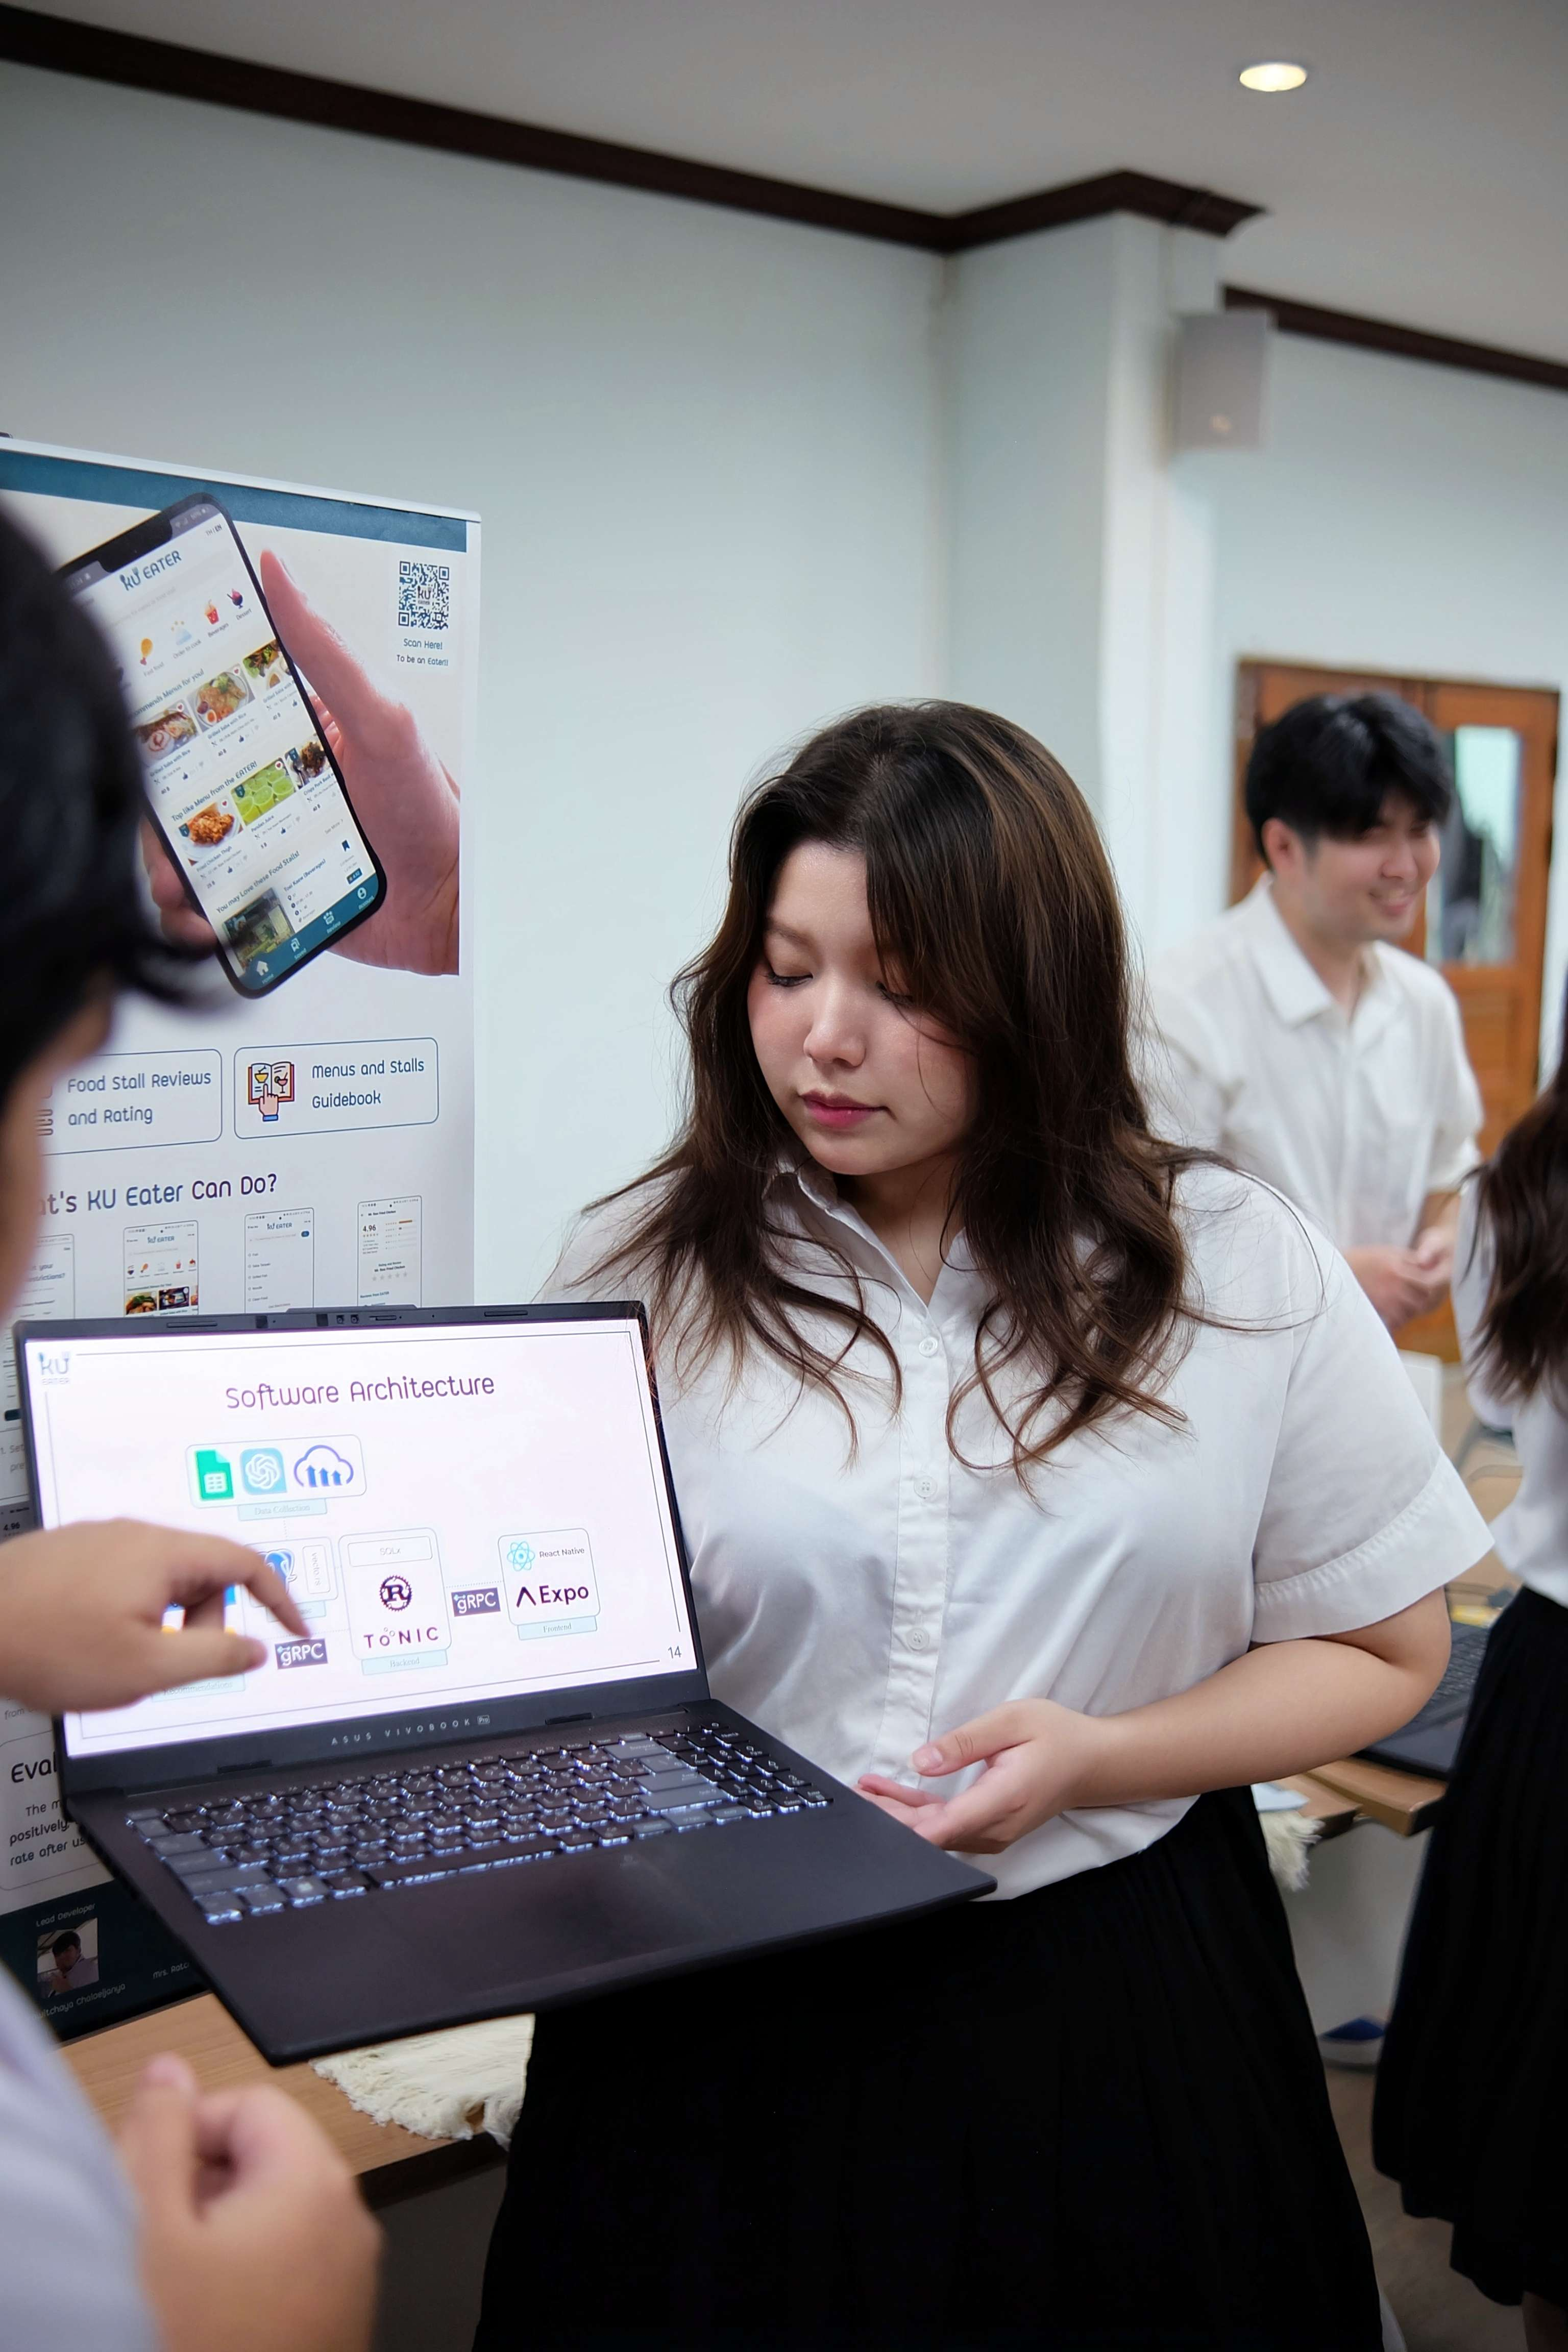
\includegraphics[height=0.4\textheight,keepaspectratio]{kueater/expo/proud.jpg}
    \end{minipage}%
    \begin{minipage}{.5\textwidth}
        \centering
        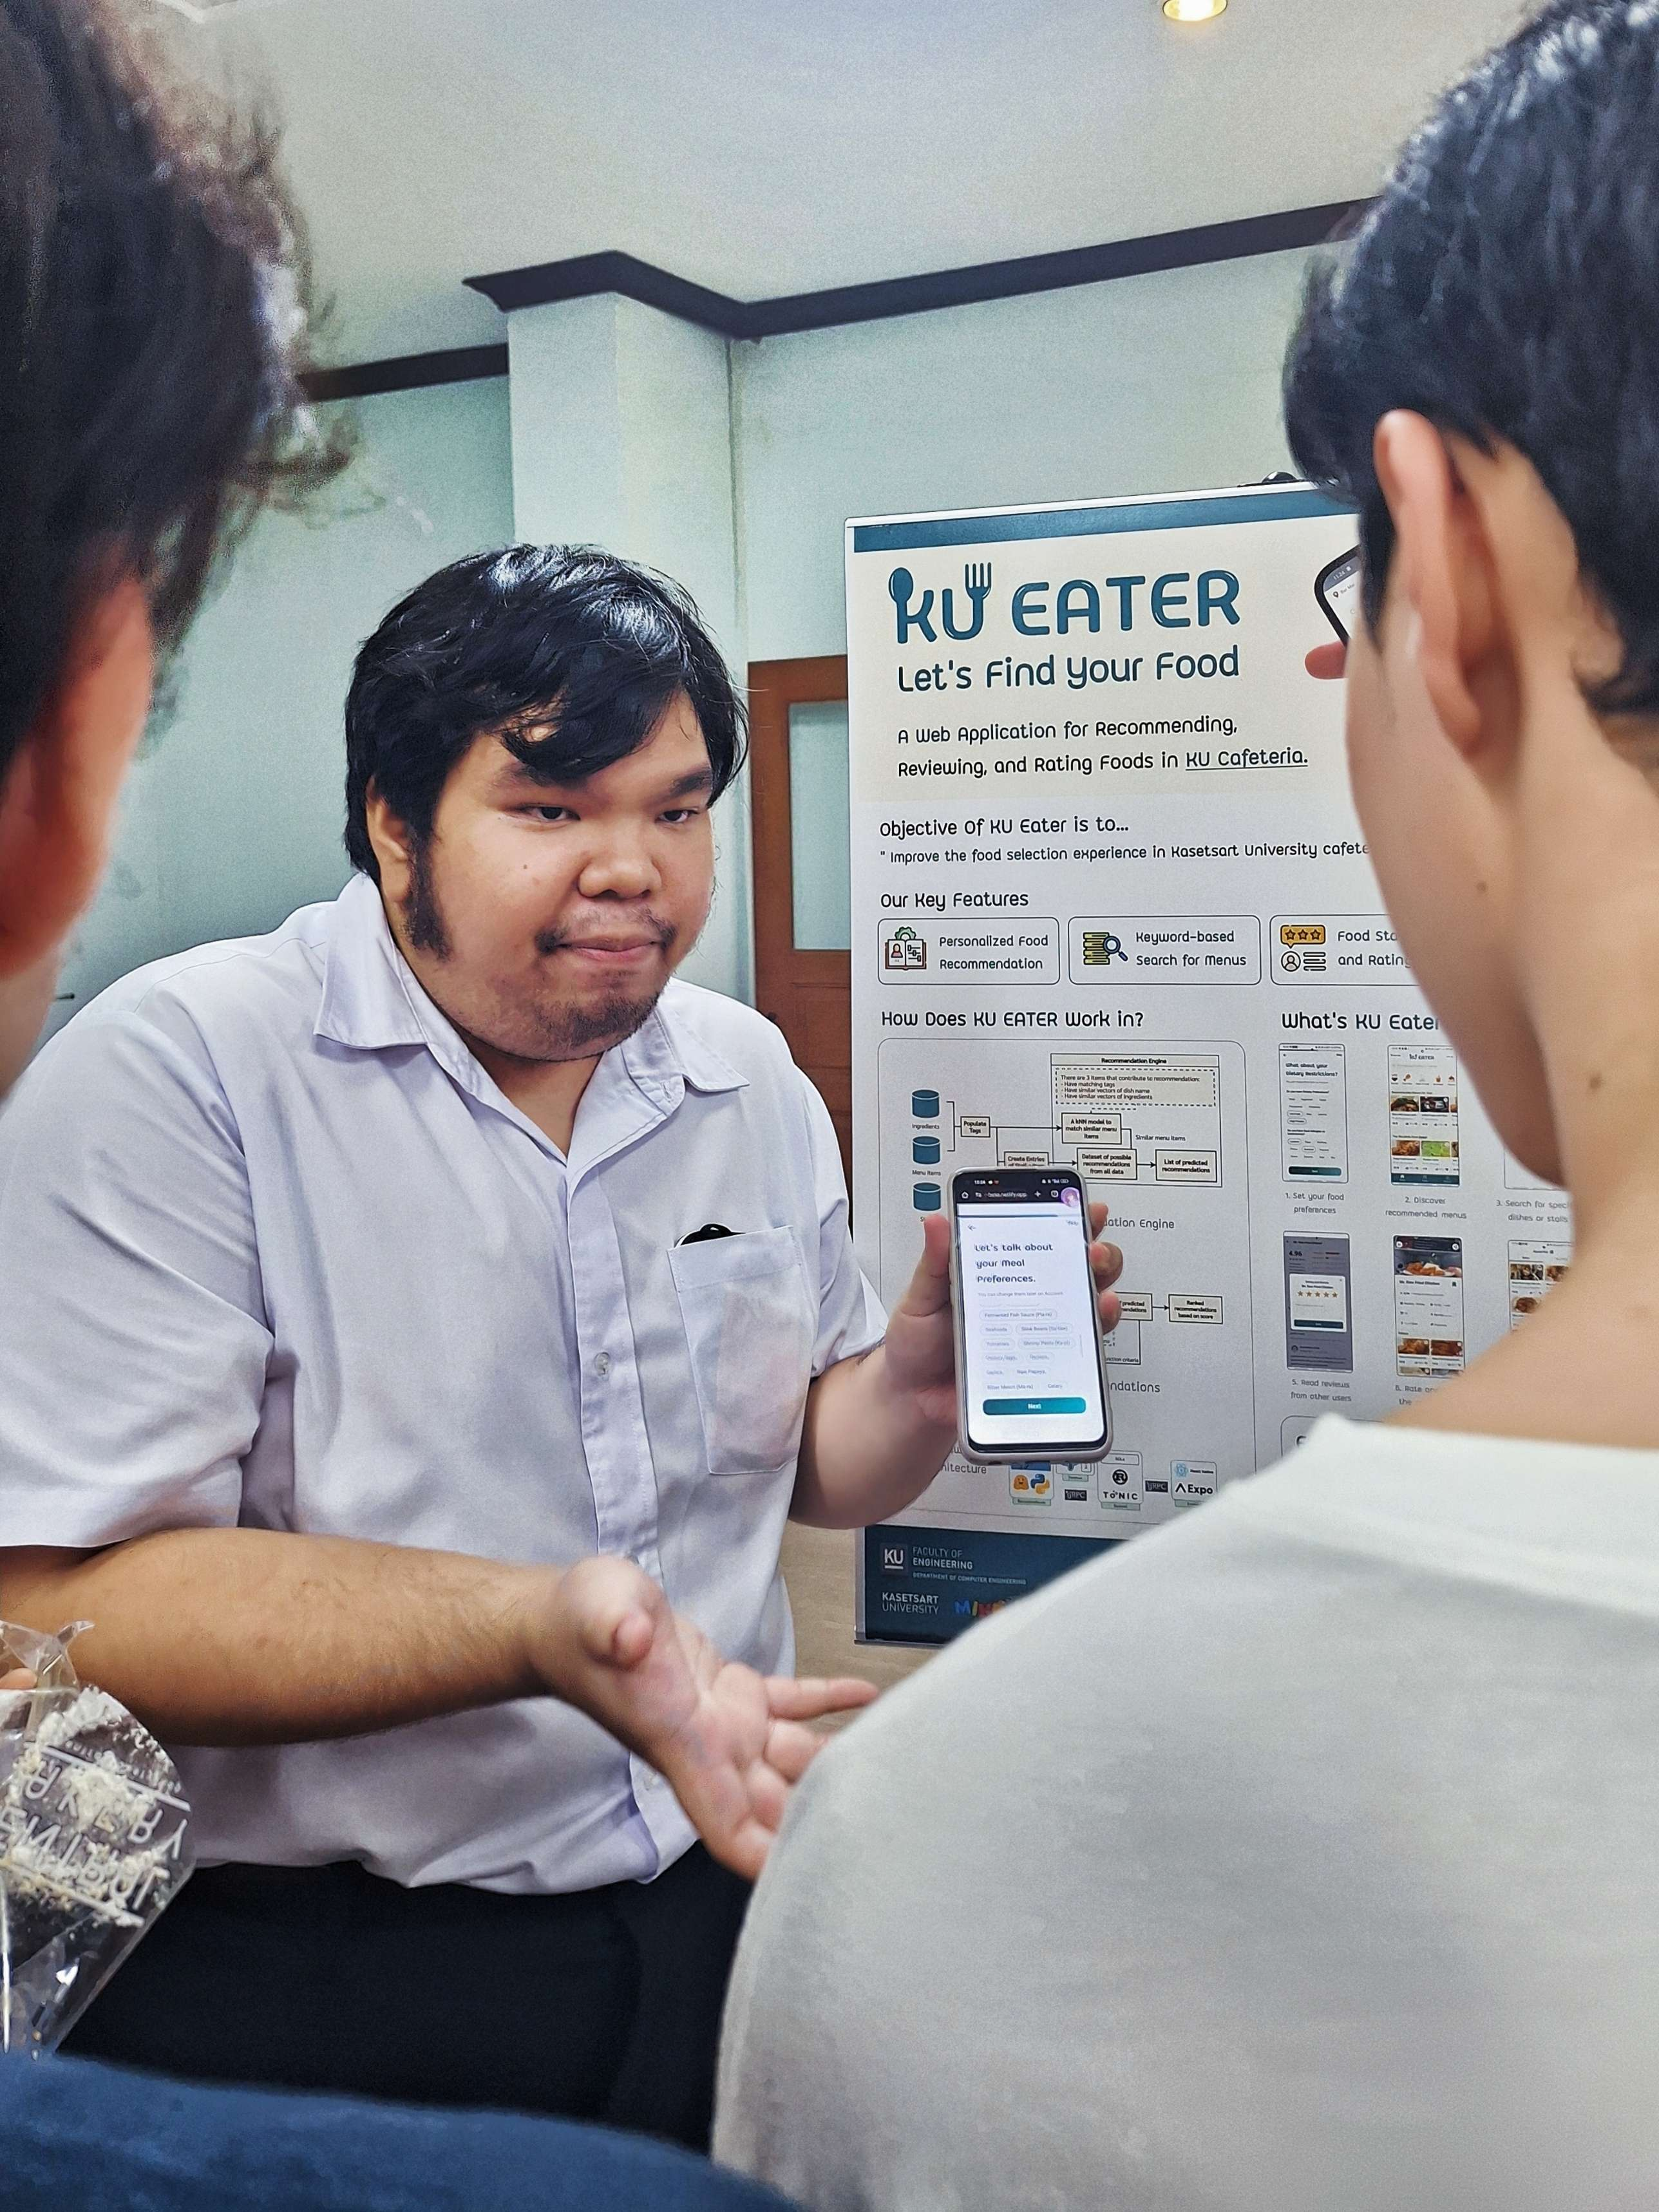
\includegraphics[height=0.4\textheight,keepaspectratio]{kueater/expo/float.jpg}
    \end{minipage}
    \caption{The members presenting the project}
    \vspace*{-\baselineskip}
\end{figure}

\section{Future Plans}
\label{section:future-plans}
Future Plans
The team intends to continue maintaining and enhancing the KU Eater application for at least one more year. Several features have been planned to increase engagement, scalability, and system sustainability:
\begin{itemize}[leftmargin=40pt]
    \item Multi-language support
    \item Menu-specific reviews and image upload
    \item Ability to change cafeteria location
    \item Backend system for stall owners to update their own menu and photos
    \item Crowdsourcing menu information from students, potentially with incentives
    \item Event promotion modal displayed at app launch
    \item Integration of monetization options such as ads or sponsorships
    \item Guest mode support for non-logged-in users
    \item Social sharing (share menu/stall links)
    \item My Reviews feature allowing users to edit or delete their past reviews
\end{itemize}

\section{Conclusion}
\label{section:conclusion-project}
KU Eater successfully fulfills its objective of improving the food selection experience at Kasetsart University cafeterias. Through a combination of intelligent recommendation, intuitive search, thoughtful design, and real user feedback, the system offers a practical and engaging tool for students navigating daily food choices. Although several challenges arose during development, each was met with a thoughtful solution that contributed to the team's growth and the project's overall success.